\section{User Interface}

\begin{figure}[H]
    \centering
    \includegraphics[scale=0.25]{imgs/UserInterface.png}
    \caption{Landing Page of the User}
\end{figure}

\subsection{Linked Resources}

\textbf{GitHub URL}: https://github.com/wdlnph/coviddb

\textbf{Live Site URL}: https://ydc353.encs.concordia.ca/coviddb/portal

\subsection{Backend Component: Laravel}

The COVID-DB Application was built by our team using the Laravel PHP Framework, built by Taylor Otwell in June 2011. Not only does it help with proper session handling, password encryption and security layers for our service, but it also provides an simple organized MVC directory layout where we can properly separate our back-end component from the front end one. This allowed for the team to be highly effective during implementation, as the Controllers would be able to be implemented concurrently to the UI Layouts to be built

To accommodate with the requirements provided to us, some compromises were made to omit the use of some features in Laravel.

\textbf{Fluent Language}

Rather than using the fluent language, we have opted to write direct SQL into our service, allowing for the marker to properly verify that the queries have been implemented

\textbf{Migrations}

A new file create\_tables.sql was created in /database/sql folder to provide all the Relations that were created throughout this project, rather than the turnkey migration solution commonly performed in Laravel.

\textbf{Seeding}

Factory files were also omitted. Instead, we have provided the files insert\_statements.sql, insert\_regions.sql and triggers.sql to ensure the database is populated in the way it should match results found in this report.

\subsection{Frontend Component: ReactJS}

For a highly intuitive interface, we have opted to make use of the ReactJS framework for our front end. React allows us to easily re-use components throughout multiple entities, and provide a simple way to validate forms and communicate with the backend component. The axios package was used to communicate with the API, and the Formik plugin is used for validation with Yup. 

In addition, we have decided to use Tailwind CSS to design our components, all of which is compiled using the Webpack wrapper provided by Laravel Mix.


\subsection{Authentication}
\\
The user is able to log in using his medicare card and password, which is its date of birth, in YYYYMMDD format. A register functionality would also be provided, as well as a forgot password and remember me checkbox. These, however, do not enter into the scope of this project.

\begin{figure}[H]
    \centering
    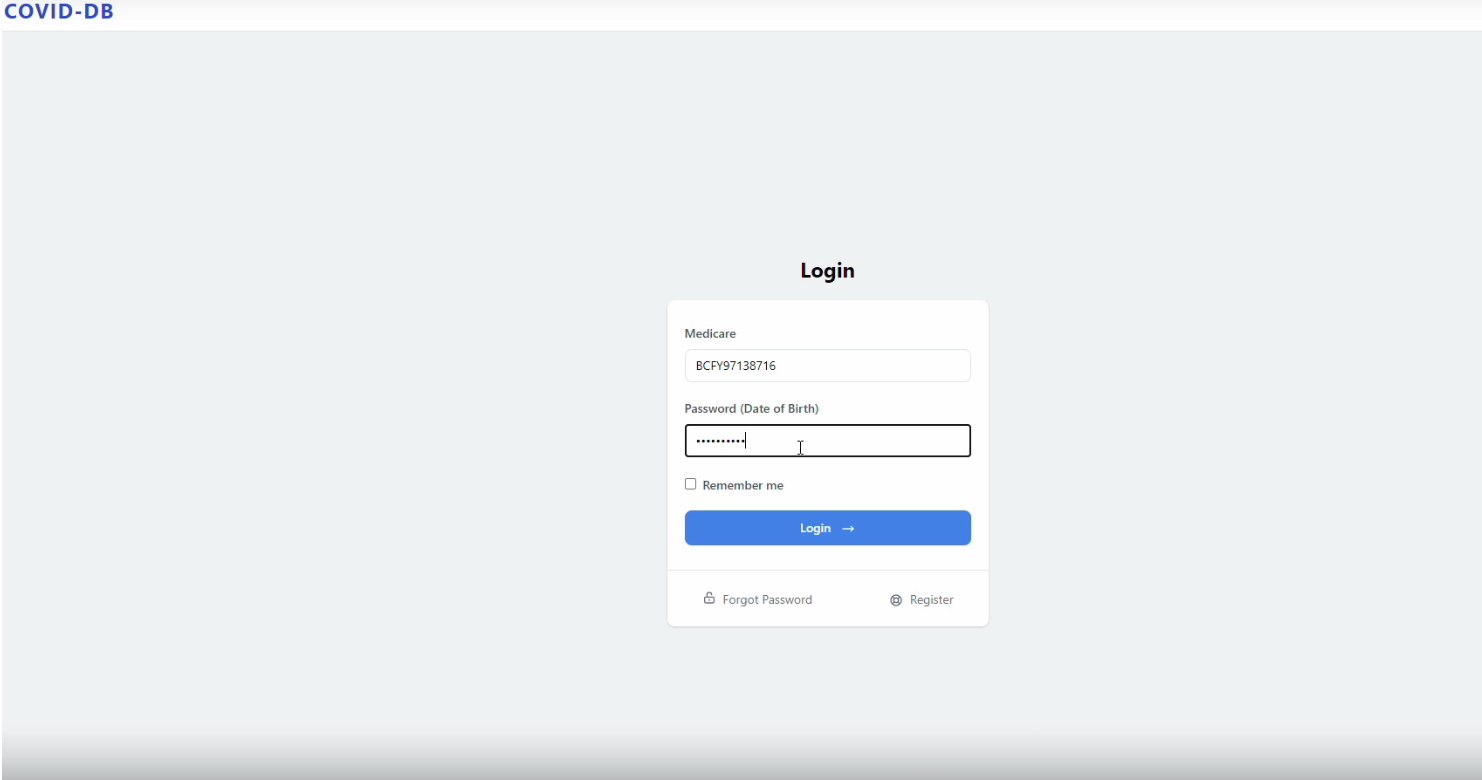
\includegraphics[scale=0.35]{imgs/loginScreen.PNG}
    \caption{Home Page allows you to login with your medicare and dob}
\end{figure}

\subsection{CRUD Table}

A table was designed to display information coming from any `readAll` functions. These rows can be clicked to further go into the Edit Entity page in order to update the selected row. Depending on the page, some filters may be provided at the top of the page.

\begin{figure}[H]
    \centering
    \includegraphics[scale=0.25]{imgs/CRUDTable.png}
    \caption{List of all workers in a table}
\end{figure}

\subsection{Create/Update Entity}

Each entity provides its own schema that can be validated using the combination of the Yup and Formik plugins. Validation prevents for erroneous data from reaching the database, as it may not result into the right constraints being respected. This only serves as a first layer protection, since the Database and the API itself provide their own validation rules as well.

The form has been made to accommodate both the creation and update of a record. a delete option is also provided at the bottom in order to delete the entity if needed.

\begin{figure}[H]
    \centering
    \includegraphics[scale=0.25]{imgs/EditCreateUser.png}
    \caption{This edit page provides feedback on what has not been filled out by the user}
\end{figure}

\subsection{Toast notification}

The Toast plugin allows us to provide to the user any information that is pertaining to him if they come to be.


\begin{figure}[H]
    \centering
    \includegraphics[scale=0.25]{imgs/Toast.png}
    \caption{A toast notification}
\end{figure}


\subsection{Region Update}

We have made the assumption that a Region cannot be deleted. Therefore, this leaves only the ability for us to update the alert level. We have therefore taken the liberty to provide a more in depth view that explains some restrictions related to the alert in place. This information can be toggled, however the information is hard coded into the application rather than in the database.

\begin{figure}[H]
    \centering
    \includegraphics[scale=0.25]{imgs/EditRegion.png}
    \caption{Edit Region Form}
\end{figure}
